\documentclass[12pt, a4paper]{article}
\usepackage{amsmath}
\usepackage{enumitem}
\usepackage{float}
\usepackage[left=2cm, right=2cm, top=2cm, bottom=2cm]{geometry}
\usepackage{graphicx}
\usepackage[colorlinks, urlcolor=blue]{hyperref}
\usepackage{minted}
\usepackage{multirow}
\usepackage{siunitx}
\usepackage{tabularx}
\usepackage{xeCJK}

\renewcommand\arraystretch{1.5}
\setCJKmainfont[AutoFakeBold=1.5]{新細明體}
\setlength{\parindent}{0pt}

\renewcommand{\tabularxcolumn}[1]{m{#1}}
\newcolumntype{C}{>{\centering\arraybackslash}X}

\setminted{frame=single}

\title{
  \vspace{-1cm}
  Network Administration/System Administration\\
  (NTU CSIE, Spring 2024)\\
  Homework \#10
}
\author{\Large B12902110 呂承諺}

\begin{document}
  \maketitle
  \section{課程內容}
  \begin{enumerate}[label=(\alph*)]
    \item 5~GHz Wi-Fi uses frequencies ranging from \qty{5.15}{\giga\hertz} to
    \qty{5.35}{\giga\hertz} and \qty{5.47}{\giga\hertz} to \qty{5.895}{\giga\hertz}.
    We choose \qty{5.50}{\giga\hertz} as an average for calculation.
    \[
      \lambda = \frac{c}{f}
      = \frac{\qty{299792458}{\meter/\second}}{\qty{5.50e9}{Hz}}
      = \qty{0.0545}{\meter} = \qty{54.5}{\milli\meter}
    \]

    \item
    \[
      \frac{P_r}{P_t} = \frac{G_tG_r\lambda^2}{\left(4\pi d\right)^2}
      = \frac{1 \left(1\right) \left(0.0545\right)^2}{\left(4\pi \left(1\right) \right)^2}
      = \num{1.88e-5}
    \]

    \item For a certain wavelength $\lambda$, suppose only the distance changes, while
    all other factors remain the same.
    \[
      P_r = \frac{P_t G_t G_r \lambda^2}{\left(4 \pi d\right)^2} \propto \frac{1}{d^2}
    \]
    This shows that both 2.4~GHz and 5~GHz signals attenuate by the same factor.

    \item Suppose the wavelength is the only changing factor.
    \[
      P_r = \frac{P_t G_t G_r \lambda^2}{\left(4 \pi d\right)^2} \propto \lambda^2
    \]
    A 2.4~GHz wave have a longer wavelength than a 5~GHz wave, so 2.4~GHz gets a stronger
    signal.

    \item Bandwidth refers to the maximum data transfer rate of the connection, while
    throughput refers to the actual data transfer rate.
  \end{enumerate}

  \textbf{References}
  \begin{footnotesize}
    \begin{itemize}
      \item \href{https://en.wikipedia.org/wiki/Wi-Fi}{Wi-Fi - Wikipedia}
      \item \href{https://en.wikipedia.org/wiki/List_of_WLAN_channels}{List of WLAN channels - Wikipedia}
      \item \href{https://en.wikipedia.org/wiki/Friis_transmission_equation}{Friis transmission equation - Wikipedia}
      \item \href{https://cool.ntu.edu.tw/courses/33591/files/5577514}{Lecture slides "Wireless Communications \& Networking" by Professor Michael Tsai, page 12}
      \item \href{https://en.wikipedia.org/wiki/Bandwidth_(signal_processing)}{Bandwidth (signal processing) - Wikipedia}
      \item \href{https://en.wikipedia.org/wiki/Bandwidth_(computing)}{Bandwidth (computing) - Wikipedia}
      \item \href{https://blog.pichuang.com.tw/20190527-bandwidth-and-throughput.html}{Bandwidth \& Throughput - 魂系架構 Phil's Workspace}
      \item \href{https://en.wikipedia.org/wiki/Network_throughput}{Network throughput - Wikipedia}
    \end{itemize}
  \end{footnotesize}

  \section{討論題}
  \begin{enumerate}[label=(\alph*)]
    \item \phantom{}\vspace{-\baselineskip}

    \begin{tabularx}{0.96\textwidth}{|
        >{\centering\arraybackslash}m{10ex}
        >{\centering\arraybackslash}m{16ex}
        >{\centering\arraybackslash}m{11.5ex}
        >{\centering\arraybackslash}m{10ex}
        >{\centering\arraybackslash}m{16.5ex}
        C|}
      \hline
      \textbf{Protocol} & \textbf{Cryptographic algorithm} & \textbf{Algorithm secure} &
      \textbf{Integrity check} & \textbf{Authentication methods} & \textbf{Possible attacks} \\\hline
      WEP & RC4 & Weak & CRC-32 & 64-bit key & Fluhrer, Mantin and Shamir attack \\\hline
      WPA & RC4+TKIP & Weak & Michael &
      \multirow[c]{2}{16.5ex}[-8pt]{\centering Personal (PSK)\newline Enterprise (802.1X)} &
      NOMORE attack \\\cline{1-4}\cline{6-6}
      WPA2 & AES-128 & Strong & CCMP && Krack attack \\\hline
      WPA3 & AES-128 or AES-256 & Strong & CCMP & Personal (SAE)\newline Enterprise (802.1X) & FragAttacks \\\hline
    \end{tabularx}

    \vspace{\baselineskip}
    \textbf{WEP} Originally proposed to provide the same level of security as wired
    networks. Uses the RC4 encryption algorithm, which is insecure today.

    \textbf{WPA} Introduces TKIP to patch the flaws in WEP due to RC4. Also adds a
    Message Integrity Check function named Michael. However, WPA still relies on weaknesses
    in WEP, making it still vulnerable to attacks.

    WPA also adds enterprise mode authentication which authenticates via a 802.1X server.

    \textbf{WPA2} Introduces AES-128 and CCMP to replace RC4, TKIP, and Michael, enhancing
    security. Though attack methods have been discovered, they can be avoided by firmware
    updates. The cryptographic algorithms are considered strong according to today's standards.

    \textbf{WPA3} Further enhances security by mandating AES-128 and CCMP
    as the minimum encryption algorithm in WPA3-Personal, and supporting AES-256 in
    WPA3-Enterprise. In addition, it replaces PSK in WPA and WPA2 with SAE for more secure
    key exchange.

    \vspace{\baselineskip}
    \textbf{References}
    \begin{itemize}
      \item \href{https://docs.google.com/presentation/d/1U6Ig4Oqgw1llAwnJMaGWxHvsajcHfcH-jbcnrQIv6LE/edit?usp=sharing}{Lab 10 Slides}
      \item \href{https://en.wikipedia.org/wiki/Wired_Equivalent_Privacy}{Wired Equivalent Privacy - Wikipedia}
      \item \href{https://en.wikipedia.org/wiki/Wi-Fi_Protected_Access}{Wi-Fi Protected Access - Wikipedia}
      \item \href{https://en.wikipedia.org/wiki/CCMP_(cryptography)}{CCMP (cryptography) - Wikipedia}
      \item \href{https://www.fragattacks.com/}{FragAttacks: Security flaws in all Wi-Fi devices}
    \end{itemize}

    \pagebreak
    \item \phantom{}\vspace{-\baselineskip}

    \begin{tabularx}{0.93\textwidth}{|
        >{\centering\arraybackslash}m{11.5ex}
        >{\centering\arraybackslash}m{11.5ex}
        >{\centering\arraybackslash}m{11.5ex}
        >{\centering\arraybackslash}m{11.5ex}
        C|}
      \hline
      \textbf{Generation} & \textbf{IEEE 802.11 standard} & \textbf{Radio frequency (GHz)} &
      \textbf{Theoretical transfer speed (Mbps)} & \textbf{New features} \\\hline
      Wi-Fi 5 & 802.11ac & 5 & 433–6933 &
      \begin{itemize}
        \item Mandatory \qty{80}{\mega\hertz} and optional \qty{160}{\mega\hertz} channel bandwidth
        \item 256-QAM
        \item Up to 8 MIMO spatial streams
        \item MU-MIMO up to 4 downlink clients
      \end{itemize} \\\hline
      Wi-Fi 6 & 802.11ax & 2.4 and 5 & 574–9608 &
      \begin{itemize}
        \item Orthogonal frequency-division multiple access (OFDMA)
        \item 1024-QAM
        \item Both downlink and uplink MU-MIMO
      \end{itemize} \\\hline
      Wi-Fi 6E & 802.11ax & 6 & 574–9608 &
      Wi-Fi 6 capabilities in the \qty{6}{\giga\hertz} band \\\hline
    \end{tabularx}

    \vspace{\baselineskip}
    \textbf{References}
    \begin{itemize}
      \item \href{https://en.wikipedia.org/wiki/IEEE_802.11ac-2013}{IEEE 802.11ac-2013 - Wikipedia}
      \item \href{https://en.wikipedia.org/wiki/Wi-Fi_6}{Wi-Fi 6 - Wikipedia}
    \end{itemize}

    \pagebreak
    \item  \phantom{}\vspace{-\baselineskip}

    \begin{tabularx}{0.93\textwidth}{|CCCCC|}
      \hline
      \textbf{Frequency band (GHz)} & \textbf{Transfer speed} & \textbf{Congestion} &
      \textbf{Coverage} & \textbf{Ease of blockage} \\\hline
      2.4 & Slowest & Most  & Best   & Hardest \\\hline
      5   & Faster  & More  & Better & Easier  \\\hline
      6   & Fastest & Least & Worst  & Easiest \\\hline
    \end{tabularx}

    More and more applications nowadays demand higher network throughput and lower latency,
    which leads to the need of a broader spectrum.
    The \qty{6}{\giga\hertz} band ranges from \qty{5.925}{\giga\hertz} to
    \qty{7.125}{\giga\hertz}, providing a wide and contiguous frequency band that
    supports up to 7 non-overlapping channels, making it suitable for high-throughput
    applications.

    Also, as the number of devices have grown substantially, the \qty{5}{\giga\hertz} may
    face congestion in populated areas. Therefore we need to open up more frequency bands
    to minimize congestion.

    \textbf{References}
    \begin{itemize}
      \item \href{https://www.intel.com/content/www/us/en/products/docs/wireless/2-4-vs-5ghz.html}{2.4 GHz vs. 5 GHz vs. 6 GHz: What's the Difference? - Intel}
      \item \href{https://www.netgear.com/hub/wifi/routers/difference-2-4-ghz-5-ghz-and-6-ghz/}{2.4 GHz vs 5 GHz vs 6 GHz WiFi: Which is Right for You?}
      \item \href{https://www.pcmag.com/news/what-is-wi-fi-6e}{What Is Wi-Fi 6E? | PCMag}
      \item \href{https://www.tp-link.com/tw/blog/164/wi-fi-6e-%E4%B8%AD%E7%9A%84-6g-%E9%A0%BB%E6%AE%B5%E4%BB%8B%E7%B4%B9-%E5%85%A9%E5%80%8D%E9%A0%BB%E5%AF%AC%E5%85%A9%E5%80%8D%E7%AA%81%E7%A0%B4/}{Wi-Fi 6E 中的 6G 頻段介紹 - 兩倍頻寬兩倍突破 | TP-Link 台灣地區}
    \end{itemize}

    \item  \phantom{}\vspace{-\baselineskip}

    \begin{tabularx}{0.93\textwidth}{|
        >{\centering\arraybackslash}m{20ex}
        >{\centering\arraybackslash}m{25ex}
        C|}
      \hline
      \textbf{Mode} & \textbf{Suitable scenarios} & \textbf{Reason} \\\hline
      Standalone mode & Smaller amount of APs (e.g., home) &
      \begin{itemize}
        \item No additional cost for AP controller
        \item Easier setup
      \end{itemize} \\\hline
      Controller mode & Larger amount of APs (e.g., business, school) &
      \begin{itemize}
        \item Centralized management, e.g., possible to deploy configuration changes to lots of APs
        \item Scalability: Easier to add new APs
      \end{itemize} \\\hline
    \end{tabularx}
  \end{enumerate}

  \pagebreak
  \section{問答題}
  \begin{enumerate}[label=(\alph*)]
    \item SSID
    \begin{enumerate}[label=(\arabic*)]
      \item SSID stands for service set identifier. It is typically the network name that
      users see.

      BSSID stands for basic service set identifier. It is usually the MAC address of the
      access point.

      One extended service set (ESS), identified by an SSID, may consist of one or
      more access points. Each access point has its own BSSID.

      \item An AP can provide service of several SSIDs simultaneously. Most home APs today
      can deploy a main SSID and another guest SSID. Another example is using different SSIDs
      for 2.4~GHz and 5~GHz signals from the same AP.

      Different APs can share the same SSID. Just configure the APs to the same SSID. This is
      exactly how the \verb|csie| Wi-Fi works in the department.

      \item An evil twin is a malicious Wi-Fi AP that mimics a legitimate one, often
      set up to have the same SSID as a public Wi-Fi and a fake login page. When a device
      automatically connects to the AP, the attacker can start monitoring the victim's
      traffic and extract sensitive information.

      We can prevent the evil twin attack by not connecting to public or insecure
      Wi-Fi, and by using secure application protocols such as SSH or HTTPS.

      \item The device will often choose the AP with the best signal quality or the first
      one that it connected to. Standards 802.11k, 802.11v, and 802.11r facilitate transition
      between basic service sets.
    \end{enumerate}
    \textbf{References}
    \begin{itemize}
      \item \href{https://en.wikipedia.org/wiki/Service_set_(802.11_network)}{Service set (802.11 network) - Wikipedia}
      \item \href{https://en.wikipedia.org/wiki/Evil_twin_(wireless_networks)}{Evil twin (wireless networks) - Wikipedia}
      \item \href{https://usa.kaspersky.com/resource-center/preemptive-safety/evil-twin-attacks}{What is an Evil Twin Attack? Evil Twin Wi-Fi Explained}
      \item \href{https://learn.microsoft.com/en-us/windows-hardware/drivers/network/fast-roaming-with-802-11k--802-11v--and-802-11r}{Fast Roaming with 802.11k, 802.11v, and 802.11r - Windows drivers | Microsoft Learn}
    \end{itemize}

    \item I would place the new AP at the front-left of the classroom, as its the
    farthest to both existing APs.

    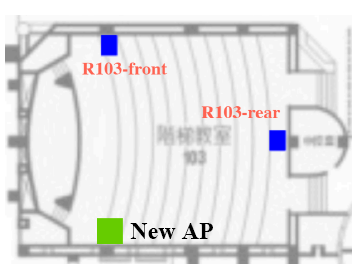
\includegraphics[width=0.4\textwidth]{3-b_new_ap.png}
  \end{enumerate}

  \section{實作題}
  The answers below are based on Windows 10.
  \begin{enumerate}[label=(\alph*)]
    \item \textbf{Steps}
    \begin{enumerate}[label=(\arabic*)]
      \item If this is the first time connecting to the Wi-Fi, we need to create a profile in
      XML format. Here we use a WPA3-Personal profile as an example.
      \inputminted[fontsize=\footnotesize]{xml}{Ultramarine.xml}
      Then we add it to the system.
      \begin{Verbatim}[frame=single]
netsh wlan add profile filename=Ultramarine.xml
      \end{Verbatim}
      \item Connect to the Wi-Fi with the following command.
      \begin{Verbatim}[frame=single]
netsh wlan connect name=Ultramarine
      \end{Verbatim}
    \end{enumerate}
    \textbf{Result}

    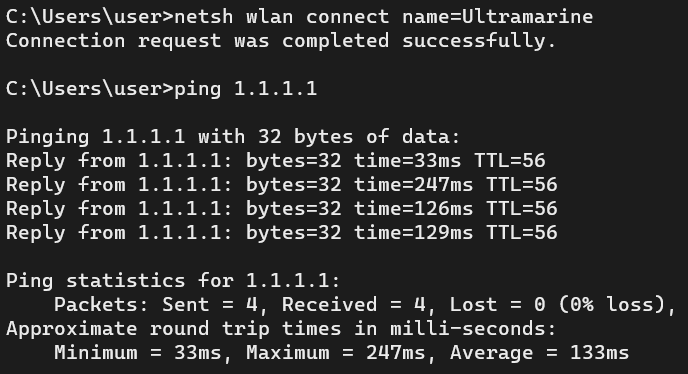
\includegraphics[width=0.6\textwidth]{4-a_netsh.png}

    \pagebreak
    \textbf{References}
    \begin{itemize}
      \item \href{https://www.windowscentral.com/how-connect-wi-fi-network-windows-10}{How to connect to a Wi-Fi network on Windows 10 | Windows Central}
      \item \href{https://stackoverflow.com/questions/32760356/how-to-connect-to-a-wifi-in-powershell-knowing-the-ssid-and-password}{How to connect to a wifi in powershell knowing the SSID and password? - Stack Overflow}
      \item \href{https://learn.microsoft.com/en-us/windows/win32/nativewifi/wpa2-personal-profile-sample}{WPA2-Personal profile sample - Win32 apps | Microsoft Learn}
    \end{itemize}

    \item \verb|csie| and \verb|csie-5g| both use WPA2-Enterprise, type PEAP. This can be seen
    under network properties in Windows' settings.

    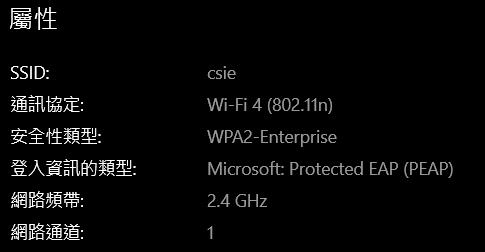
\includegraphics[width=0.5\textwidth]{4-b_csie.png}

    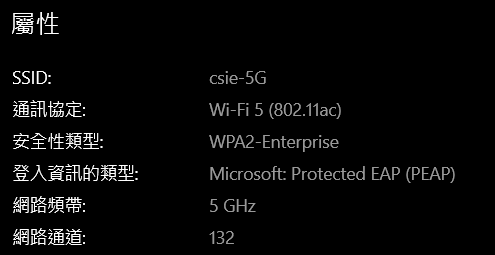
\includegraphics[width=0.5\textwidth]{4-b_csie-5G.png}
  \end{enumerate}
\end{document}
